%\documentclass[varwidth,border=0pt]{standalone}
\documentclass[varwidth,convert={density=500,outext=.png},border=0pt]{standalone}

% Tikz packages
\usepackage{tikz}
\usetikzlibrary{%
  patterns, plotmarks, backgrounds, shapes, arrows, calc, trees, positioning,
  chains, shapes.geometric, decorations.pathreplacing,
  decorations.pathmorphing, shapes.arrows, decorations.markings, quotes,
  arrows.meta, spy, fit, matrix
}

% General includegraphics and colour support
\usepackage{graphicx}
\usepackage{xcolor}
% Captions and subcaptions
\usepackage{caption}
\usepackage[labelformat=parens]{subcaption}

% String macros (for reading in tabular data)
\usepackage{xstring}

% PGFPlots
\usepackage{pgfplots}
\usepackage{pgfplotstable}
\pgfplotsset{%
  compat=newest,
  plot coordinates/math parser=false
}

%% Define node types
\tikzstyle{lnode} = [%
  circle,
  draw=black,
  minimum height=0.65cm,
  align=center,
  fill=none,
  text centered,
  inner sep=0.5pt,
  font=\tiny
]%

\begin{document}
  \begin{figure}
    \centering
    \scalebox{0.75}{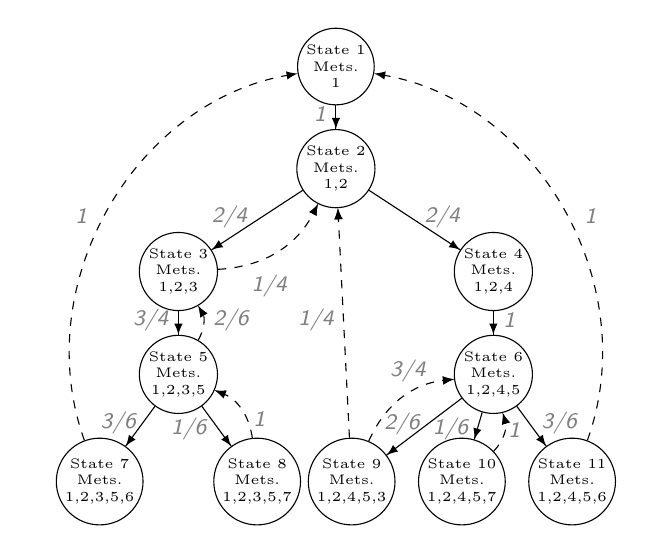
\begin{tikzpicture}[%
  >=latex,
  decoration={%
    markings,
    mark=at position 1.0 with {\arrow{>}}
  },
  every node/.style={%
    font=\sffamily\footnotesize\itshape,
    text=gray,
    text centered,
    align=center
  },
  frame/.style={draw=black,inner sep=2pt}
]

  % Nodes
  \node[lnode,text=black] (A1) {State 1\\Mets.\\1};
  \node[lnode,text=black,below=0.3cm of A1] (A2) {State 2\\Mets.\\1,2};
  \node[lnode,text=black,below=0.3cm of A2,xshift=-2.0cm] (A3) {State 3\\Mets.\\1,2,3};
  \node[lnode,text=black,below=0.3cm of A2,xshift=+2.0cm] (A4) {State 4\\Mets.\\1,2,4};
  \node[lnode,text=black,below=0.3cm of A3] (A53) {State 5\\Mets.\\1,2,3,5};
  \node[lnode,text=black,below=0.3cm of A53,xshift=-1.0cm] (A653) {State 7\\Mets.\\1,2,3,5,6};
  \node[lnode,text=black,below=0.3cm of A53,xshift=+1.0cm] (A753) {State 8\\Mets.\\1,2,3,5,7};
  \node[lnode,text=black,below=0.3cm of A4] (A54) {State 6\\Mets.\\1,2,4,5};
  \node[lnode,text=black,below=0.3cm of A54,xshift=-1.8cm] (A34) {State 9\\Mets.\\1,2,4,5,3};
  \node[lnode,text=black,below=0.3cm of A54,xshift=-0.4cm] (A74) {State 10\\Mets.\\1,2,4,5,7};
  \node[lnode,text=black,below=0.3cm of A54,xshift=+1.0cm] (A64) {State 11\\Mets.\\1,2,4,5,6};

  % Intra-node edges
  \draw[postaction={decorate}] (A1) to node [left=0.1pt,yshift=1pt] {1} (A2);
  \draw[postaction={decorate}] (A2) to node [left=0.1pt,yshift=1pt] {2/4} (A3);
  \draw[postaction={decorate}] (A2) to node [right=0.1pt,yshift=1pt] {2/4} (A4);
  \draw[postaction={decorate}] (A3) to node [left=0.1pt,yshift=1pt] {3/4} (A53);
  \draw[postaction={decorate}] (A53) to node [left=0.1pt,yshift=1pt,xshift=2pt] {3/6} (A653);
  \draw[postaction={decorate}] (A53) to node [left=0.1pt,yshift=-1pt] {1/6} (A753);
  \draw[postaction={decorate}] (A4) to node [right=0.1pt,yshift=1pt] {1} (A54);
  \draw[postaction={decorate}] (A54) to node [left=0.1pt,yshift=1pt,xshift=2pt] {2/6} (A34);
  \draw[postaction={decorate}] (A54) to node [left=0.1pt,yshift=-1pt] {1/6} (A74);
  \draw[postaction={decorate}] (A54) to node [right=0.1pt,yshift=1pt] {3/6} (A64);

  % EFM edges
  \draw[dashed,->,postaction={decorate}] (A3) to [bend right=30] node [below right=0.1pt,yshift=-5pt,xshift=-13pt] {1/4} (A2);
  \draw[dashed,->,postaction={decorate}] (A34) to [bend left=0] node [left=0.1pt,yshift=+1pt] {1/4} (A2);
  \draw[dashed,->,postaction={decorate}] (A753) to [bend right=30] node [right=0.1pt,xshift=+1pt,yshift=-4pt] {1} (A53);
  \draw[dashed,->,postaction={decorate}] (A53) to [bend right=30] node [right=0.1pt,yshift=+1pt] {2/6} (A3);
  \draw[dashed,->,postaction={decorate}] (A74) to [bend right=30] node [right=0.1pt,yshift=+1pt,xshift=-2pt] {1} (A54);
  \draw[dashed,->,postaction={decorate}] (A34) to [bend left=30] node [above=0.1pt,yshift=+2pt,xshift=2pt] {3/4} (A54);
  \draw[dashed,->,postaction={decorate}] (A653) to [bend left=50] node [left=4.3pt,yshift=-0.09cm] {1} (A1);
  \draw[dashed,->,postaction={decorate}] (A64) to [bend right=50] node [right=4.3pt,yshift=-0.09cm] {1} (A1);

\end{tikzpicture}

}
    %\vspace*{-1.18em}
  \end{figure}
\end{document}


